\documentclass[handout, 10pt, aspectratio=43]{beamer}
%\documentclass[10pt, aspectratio=43]{beamer}
%\usepackage[english]{babel}
\usepackage{amsthm}
\usepackage{animate}
\usepackage{mathtools}
\usepackage{physics}
\usepackage{calligra}
\usepackage{csquotes}
\usepackage{tensor}
\usepackage[thicklines]{cancel}
\usepackage{tcolorbox}
\usepackage{pstricks}
\usepackage{ulem}
%\usepackage[ngerman]{babel} % Language hyphenation and typographical rules
%\usepackage[backend=biber, style=numeric]{biblatex}

\setbeamersize{text margin left=0.5cm,text margin right=0.5cm}


\DeclareMathAlphabet{\mathcalligra}{T1}{calligra}{m}{n}
\DeclareFontShape{T1}{calligra}{m}{n}{<->s*[2.2]callig15}{}
\newcommand{\scriptr}{\mathcalligra{r}\,}
\newcommand{\boldscriptr}{\pmb{\mathcalligra{r}}\,}
\def\rc{\scriptr}
\def\brc{\boldscriptr}
\def\hrc{\hat\brc}
\newcommand{\ie}{\emph{i.e.}} %id est
\newcommand{\eg}{\emph{e.g.}} %exempli gratia
\newcommand{\rtd}[1]{\ensuremath{\left\lfloor #1 \right\rfloor}}
\newcommand{\dirac}[1]{\ensuremath{\delta \left( #1 \right)}}
\newcommand{\diract}[1]{\ensuremath{\delta^3 \left( #1 \right)}}
\newcommand{\e}{\ensuremath{\epsilon_0}}
\newcommand{\m}{\ensuremath{\mu_0}}
\newcommand{\V}{\ensuremath{\mathcal{V}}}
\newcommand{\prnt}[1]{\ensuremath{\left(#1\right)}} %parentheses
\newcommand{\colch}[1]{\ensuremath{\left[#1\right]}} %square brackets
\newcommand{\chave}[1]{\ensuremath{\left\{#1\right\}}}  %curly brackets

\useoutertheme{infolines}
\useinnertheme{rectangles}
\usefonttheme{professionalfonts}


%\definecolor{blue}{RGB}{0, 169, 224}
\definecolor{blue}{RGB}{0, 130, 224}
\definecolor{gray}{HTML}{ffffff}
\definecolor{yellow}{HTML}{f0be52}
\definecolor{lightblue}{RGB}{89, 199, 254}

\renewcommand{\CancelColor}{\color{blue}}

\makeatletter
\newcommand{\mybox}[1]{%
  \setbox0=\hbox{#1}%
  \setlength{\@tempdima}{\dimexpr\wd0+13pt}%
  \begin{tcolorbox}[colback=blue,colframe=blue,boxrule=0.5pt,arc=4pt,
      left=6pt,right=6pt,top=6pt,bottom=6pt,boxsep=0pt,width=\@tempdima]
    \textcolor{black}{#1}
  \end{tcolorbox}
}
\makeatother

\usecolortheme[named=blue]{structure}
\usecolortheme{sidebartab}
\usecolortheme{orchid}
\usecolortheme{whale}
\setbeamercolor{alerted text}{fg=yellow}
\setbeamercolor{block title alerted}{bg=alerted text.fg!90!black}
\setbeamercolor{block title example}{bg=lightblue!60!black}
\setbeamercolor{background canvas}{bg=gray}
\setbeamercolor{normal text}{bg=gray,fg=black}

\setbeamertemplate{footline}
        {
      \leavevmode%
      \hbox{%
      \begin{beamercolorbox}[wd=.333333\paperwidth,ht=2.25ex,dp=1ex,center]{author in head/foot}%
        \usebeamerfont{author in head/foot}\insertshortauthor~~(\insertshortinstitute)
      \end{beamercolorbox}%
      \begin{beamercolorbox}[wd=.333333\paperwidth,ht=2.25ex,dp=1ex,center]{title in head/foot}%
        \usebeamerfont{title in head/foot}\insertshorttitle
      \end{beamercolorbox}%
      \begin{beamercolorbox}[wd=.333333\paperwidth,ht=2.25ex,dp=1ex,center]{date in head/foot}%
        \usebeamerfont{date in head/foot}\insertshortdate{}%\hspace*{2em}

    %#turning the next line into a comment, erases the frame numbers
        %\insertframenumber{} / \inserttotalframenumber\hspace*{2ex} 

      \end{beamercolorbox}}%
      \vskip0pt%
    }


\setbeamertemplate{blocks}[rectangle]
\setbeamercovered{dynamic}

\setbeamertemplate{section page}
{
	\begin{centering}
		\begin{beamercolorbox}[sep=27pt,center]{part title}
			\usebeamerfont{section title}\insertsection\par
			\usebeamerfont{subsection title}\insertsubsection\par
		\end{beamercolorbox}
	\end{centering}
}

%\setbeamertemplate{subsection page}
%{
%	\begin{centering}
%		\begin{beamercolorbox}[sep=12pt,center]{part title}
%			\usebeamerfont{subsection title}\insertsubsection\par
%		\end{beamercolorbox}
%	\end{centering}
%}

\newcommand{\hlight}[1]{\colorbox{violet!50}{#1}}
\newcommand{\hlighta}[1]{\colorbox{red!50}{#1}}

\settowidth{\leftmargini}{\usebeamertemplate{itemize item}}
\addtolength{\leftmargini}{\labelsep}

\usepackage{ragged2e}
\usepackage{cases}

\mathcode`\*="8000
{\catcode`\*\active\gdef*{\cdot}}

\usepackage[]{siunitx}

\sisetup{per-mode=fraction, locale = US, expproduct = cdot }
\sisetup{locale = UK}							%	Automatische Einstellung der Ausgabe für bestimmte Regionen (UK, US, DE, FR, ZA)
\sisetup{
	per-mode=fraction,
	fraction-function=\tfrac
}
\DeclareSIUnit\Hy{H}
\DeclareSIUnit\hPa{hPa}
\DeclareSIUnit\Torr{Torr}
\DeclareSIUnit\T{T}
% FLORIAN
\usepackage{graphics}
\def\R{{\mathbb{R}}}
\def\N{{\mathbb{N}}}
\def\C{{\mathbb{C}}}
\def\K{{\mathbb{K}}}
\def\Q{{\mathbb{Q}}}
\def\Z{{\mathbb{Z}}}
\def\O{{\mathcal{O}}}
\def\Pot{{\mathcal{P}}}
\def\P{{\mathbb{P}}}
\def\D{{\mathcal{D}}}
\def\B{{\mathcal{B}}}
\def\U{{\mathcal{U}}}
\def\F{{\mathcal{F}}}
\def\M{{\mathcal{M}}}
\def\E{{\mathbb{E}}}
\def\EEE{{\mathcal{E}}}
\def\Cov{{\mathbb{C}\mathrm{ov}}}
\def\Var{{\mathbb{V}\mathrm{ar}}}
\def\V{{\mathbb{V}}}
\def\ND{{\mathcal{N}}}
\def\essup{{\mathrm{ess \;sup}}}

\usepackage{multirow}
\usepackage{booktabs}
\usepackage{subfigure}

\title{Kalte Fusion (LENR)} %->->->->-> Check hyperref title <-<-<-<-<-
\subtitle{Von wissenschaftlicher Hoffnung zur Verschwörungstheorie}
\author{Franz Herbst}
\institute[Universität Konstanz]{
    Im Rahmen der Vorlesung Kern- und Teilchenphysik \\
    Universität Konstanz
} %You can change the Institution if you are from somewhere else
\date{12. Januar 2021}
%\logo{\includegraphics[width= 0.2\textwidth]{images/a-logo.png}}

\begin{document}
    \RaggedRight
    \frame{\titlepage}
    
    \begin{frame}{Inhalt}
        \tableofcontents
    \end{frame}
    
    \section{Motivation and initial Dataset}


\begin{frame}{The \enquote{comma ai speed challenge}\footnote{https://github.com/commaai/speedchallenge}}
	\textbf{Motivation}
	\begin{itemize}
		\item autonomous driving is currently one of the most prominent problems in machine learning
		\item but quite hard to set up on a desktop pc
		\item predicting a vehicles velocity from video footage is a related but also much more simplified task
	\end{itemize}
	\pause
	\textbf{Initial Dataset:}
	\begin{itemize}
		\item training video with 20400 frames (20 fps)
		\item data file with velocity of the car at each frame
		\item test video with 10798 frames (20 fps)
	\end{itemize}
	\pause
	\textbf{Evaluation:}
	\begin{itemize}
		\item the mean squared error (MSE) is used to measure performance
		\begin{align*}
			\mathcal{L} = \sum_i (p(x_i) - y_i)^2
		\end{align*}
	\end{itemize}
\end{frame}

\begin{comment}

\begin{frame}{The \enquote{comma ai speed challenge}\footnote{https://github.com/commaai/speedchallenge}}
\textbf{Motivation}
\begin{itemize}
\item HERE ARE SOME MOTIVATIONAL WORDS NEEDED
\end{itemize}
\textbf{Data collection:}
\begin{itemize}
\item \enquote{comma ai speed challenge} provides two videos:
\setbeamertemplate{itemize items}[circle]
\begin{itemize}
\item Train video: 24000 frames, shoot at 20 frames per second, including ground truths
\item Test video: 10798 frames, shoot at 20 frames per second, no ground truths, used to applications
\end{itemize}
\item Split train video after 80$\%$ with hard cut off (ability the generalize), to get train and test datasets
\end{itemize}
\textbf{Initial assumptions}
\begin{itemize}
\item<+-> Use mean squared error (MSE) as a performance measure
\item<+-> How to evaluate a prediction? Assumptions:
\setbeamertemplate{itemize items}[circle]
\begin{itemize}
\item MSE $\leq 10$: good
\item MSE $\leq 5$: better
\item MSE $\leq 3$: correct
\end{itemize}
\end{itemize}
\end{frame}

\end{comment}
    \section{Fusionswahrscheinlichkeiten}

\begin{frame}{Fusion als Energiequelle}
    \begin{columns}
        \begin{column}{0.55\textwidth}
            \begin{itemize}
                \item<+-> Unterschiedliche Fusionen für Wasserstoffisotope
                \item<+-> Produkte: $\gamma$-Strahlung und Helium
                \item<+-> Reaktion, wenn Coulomb-Abstoßung der Kerne überwunden wird
            \end{itemize}
        \end{column}
        \begin{column}{0.45\textwidth}
            \begin{center}
                \only<1->{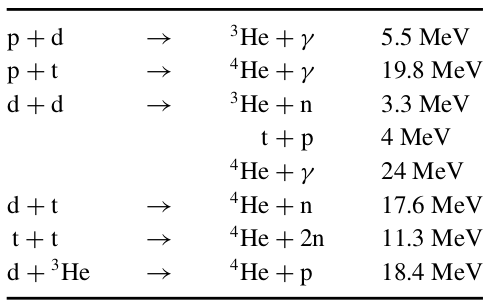
\includegraphics[width=0.75\textwidth]{images/Fusionsprozesse.png}
                \small{Interessante Fusionsprozesse mit schwerem Wasserstoff             \cite{Naga03}}}
            \end{center}
        \end{column}
    \end{columns}
    
    \only<3->{\textbf{Vorteile:}}
    \begin{itemize}
        \item<+-> Beinahe unbegrenzte Beschaffbarkeit der Rohstoffe (D, T) in Meer und Flüssen
        \item<+-> Quasi kein $\mathrm{CO_2}$-Ausstoß
        \item<+-> Kaum Produktion (langlebiger) radioaktiver Produkte
    \end{itemize}
    \only<6->{\textbf{Nachteile:}}
    \begin{itemize}
        \item<+-> Einen kontinuierlichen Fusionsprozess zu erzeugen und am Laufen zu halten ist nur schwer umsetzbar
    \end{itemize}
\end{frame}

\begin{frame}{Das Problem mit der Fusion}
    \begin{columns}
        \begin{column}{0.55\textwidth}
            \begin{itemize}
                \item<+-> Coulomb-Potential: \begin{align}V_C(r) = \frac{1}{4 \pi \varepsilon_0} \frac{q_1*q_2}{r}\end{align} Kernkräfte im Bereich $r < R_K \approx \SI{1}{\femto\m}$
                \item<+-> 2 Kerne können Barriere durch Tunneln überwinden
                \item<+-> Trotzdem erforderlich:
                \begin{itemize}
                    \item<+-> Erzeugung sehr hoher Temperaturen (Sonne)
                    \item<+-> Verwendung eines Katalysators
                \end{itemize}
            \end{itemize}
        \end{column}
        \begin{column}{0.45\textwidth}
            \begin{center}
                \only<1->{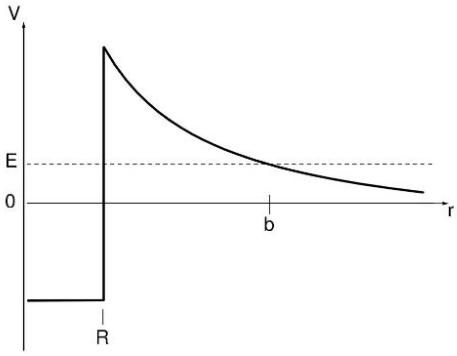
\includegraphics[width=\textwidth]{images/Potential.png}
                
                \small{Coulomb Potential \cite{IK4}}}
            \end{center}
        \end{column}
    \end{columns}
\end{frame}

\begin{frame}{Tunnelwahrscheinlichkeiten}
    \begin{itemize}
        \item<+-> Tunnelwahrscheinlichkeit mit $V(r) = \begin{cases}V_0 & \text{für } R_K < r < R_A \\ 0 & \text{sonst}\end{cases}$:
        \begin{align*}
            P \approx \frac{16 E * (V_0 - E)}{V_0^2} * \exp\left(- \frac{R_A - R_K}{\hbar} \sqrt{8m*(V_0 - E)}\right)
        \end{align*}
        \item<+-> Bestimme $V_0 = \frac{1}{R_A - R_K} \int\limits_{R_K}^{R_A} V_C(r) \mathrm{d}r$
        \begin{itemize}
            \item<+-> Plasma: $R_A$ definiert durch $E = V(R_A)$
            \item<+-> Atome: $R_A = \frac{4\pi\varepsilon_0 * \hbar^2}{m_e * e^2}$ sei durch Bohrschen Radius genähert (nur für $E < E_{ion}$)
        \end{itemize}
        \item<+-> Energie $E = \frac{3}{2} k_B T$ sei mit thermischer Energie genähert
    \end{itemize}
\end{frame}

\begin{frame}{Tunnelwahrscheinlichkeiten}
    \centering
    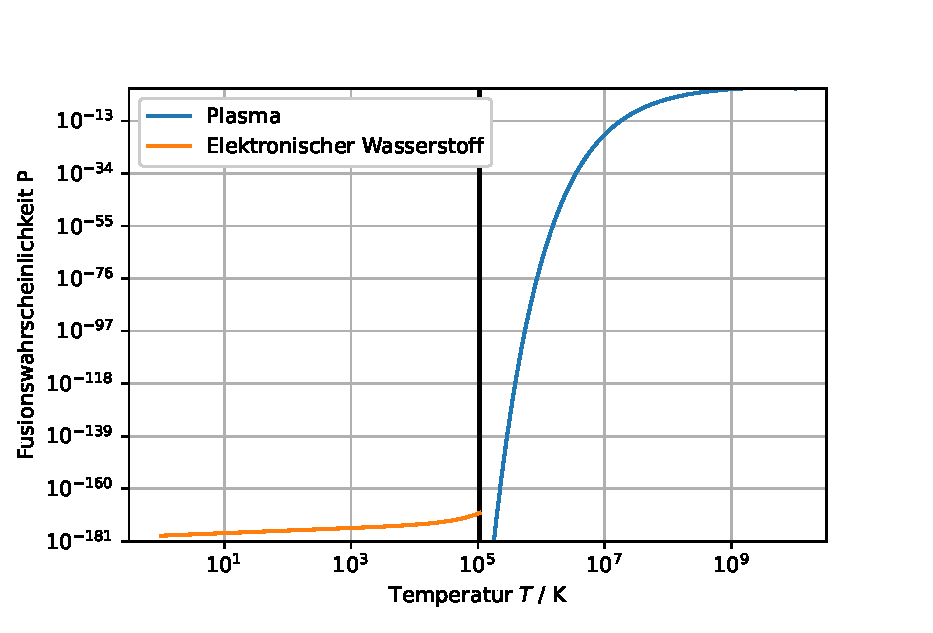
\includegraphics[width=0.8\textwidth]{images/Tunnelwahrscheinlichkeiten1.eps}
\end{frame}

    \section{Myonische Fusion}

\begin{frame}{Myonenkatalysierte Fusion}
    \begin{columns}
        \begin{column}{0.55\textwidth}
            \begin{itemize}
                \item<+-> \textbf{Myon}:
                \begin{itemize}
                    \item Ladung: $q_\mu = -1\,e$
                    \item Masse: $m_\mu = 206.768\,m_\text{e}$
                    \item Lebensdauer: $\SI{2.197e-6}{\s}$ \\
                     (Zerfällt: $\mu^- \to e^- + \overline{\nu}_e + \nu_\mu$)
                    \item Spin: $s= \frac{1}{2}$
                \end{itemize}
                \item<+-> In H/D/T-Atom oder $\text{H/D/T}_2$ kann Myon die Elektronen verdrängen
                \item<+-> ähnliche Orbitale aus wie $e^-$ Atome, aber mit vielfach geringerer räumlicher Ausdehnung
                \item<+-> Kerne kommen sich näher daher Fusion bei viel niedrigeren Temperaturen möglich
                \item<+-> Bei Fusion wird Myon wieder frei
                \item<+-> Theoretisch vorhergesagt 1947 \cite{myonTheory} und nachgewiesen 1957 \cite{myonExp}
            \end{itemize}
        \end{column}
        \begin{column}{0.45\textwidth}
            \begin{center}
                \only<2->{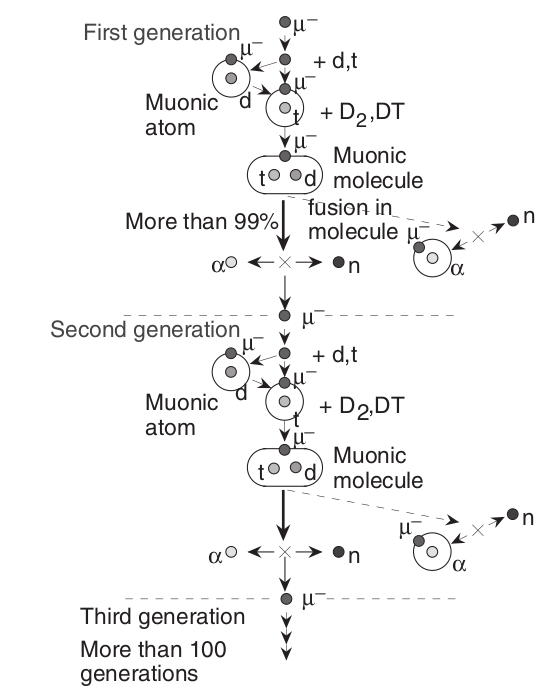
\includegraphics[width=0.9\textwidth]{images/FusionCyclus.png}
                \small{Myonischer Fusionszyklus \cite[S.71]{Naga03}}}
            \end{center}
        \end{column}
    \end{columns}
\end{frame}

\begin{frame}{Tunnelwahrscheinlichkeiten}
    \centering
    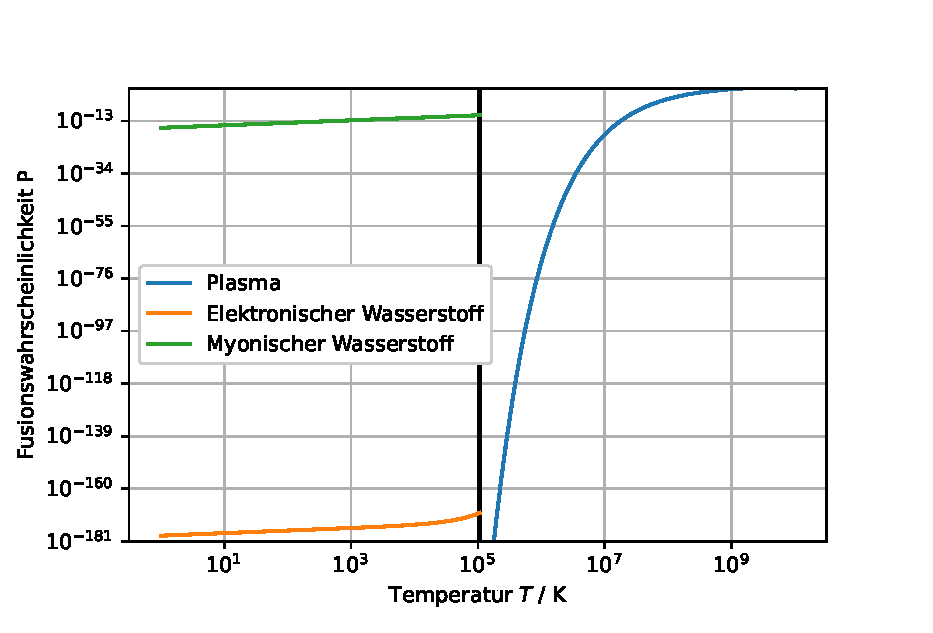
\includegraphics[width=0.8\textwidth]{images/Tunnelwahrscheinlichkeiten.eps}
\end{frame}

\begin{frame}{Energiebilanz}
    \begin{itemize}
        \item<+-> Produktion von Myonen im Teilchenbeschleuniger (z.B. $S\mu S$ Methode)
        \item<+-> Protonen werden auf C-Atome geschossen, dabei entstehen Pionen, die in Myonen zerfallen
        \item<+-> Energieaufwand im besten Fall: $\SI{-5}{\giga\eV}$ pro Myon \cite[S.93]{Naga03}
        \item<+-> Unter Vernachlässigung aller Verluste beim Transport, o.a. kann jedes Myon in etwa 150 Fusionen ermöglichen \cite[S.97]{Naga03}, bis sie
        \begin{itemize}
            \item durch Zerfall verloren gehen
            \item an ein Fusionsprodukt gebunden werden
        \end{itemize}
        \item<+-> Je nach Fusionsprozess werden zwischen $\SI{3.3}{\mega\eV}$ und $\SI{24}{\mega\eV}$ frei
        \item<+-> Energiegewinn: $\SI{3.6}{\giga\eV}$ pro Myon (für \SI{24}{\mega\eV}) \\ $\Rightarrow$ Netto Energieverbrauch
        \item<+-> Für Nutzbarkeit zur Stromerzeugung wäre ein Energiegewinn von etwa $\SI{20}{\giga\eV}$ nötig
        \item<+-> Verbesserung: Verringerung der Erzeugungsenergie der Myonen, mehr Fusionen pro Myon ermöglichen
    \end{itemize}
\end{frame}

\section{Weitere Katalysatoren}

\begin{frame}{Weitere Katalysatoren}
    \begin{itemize}
        \item<+-> \textbf{Pyrofusion:} Ionisation und Beschleunigung von Deuteriumkernen mit pyroelektrischem Kristall als Spannungsquelle. Erzeugt 400-fache der natürlichen Neutronenstrahlung. Vermutete Ursache $\mathrm{D + D} \to \ ^3\mathrm{He} + \mathrm{n}$. \\
        \underline{Aber:} Beschränkung auf geringe Teilchenströme, daher nur als Neutronenquelle nutzbar und für Energieerzeugung ungeeignet. \cite{wiki:ColdFuison}
        \item<+-> \textbf{Sonofusion:} kontrollierte Fusion durch Erzeugung von Kavitation mit Schallwellen (Science-Artikel) \\
        \underline{Aber:} Gefälschte Ergebnisse (Bubblegate) \cite{FAZ}
        \item<+-> weitere dubiose Aufbauten bei denen eine genauere Überprüfung durch dritte verweigert wurde
    \end{itemize}
\end{frame}
    \section{Zusammenfassung}

\begin{frame}{Fazit}
    \begin{itemize}
        \item<+-> Kalte Fusion ist (leider) ein wissenschaftliches Minenfeld aufgrund der großen Auswirkungen die eine erfolgreiche Durchführung hätte
        \item<+-> Mehrere Fälle mit entweder fahrlässig unsauber durchgeführten Messungen und Methoden oder sogar klarem Betrug bekannt
        \item<+-> Große Anziehungskraft auf \glqq Hobbywissenschaftler\grqq und Verschwörungs- theoretiker (vgl. YouTube)
        \item<+-> Einzige seriöse bisher bekannter Prozess der theoretisch zur Energieerzeugung geeignet wäre ist myonisch katalysierte Fusion
        \item<+-> Sehr interessantes Forschungsgebiet (vgl. \cite{Naga03})
        \item<+-> Jedoch auch hier nicht in kurzer Zeit mit einem Durchbruch zu rechnen
    \end{itemize}
\end{frame}

\begin{frame}{Zusammenfassung}
    \begin{columns}
        \begin{column}{0.6\textwidth}
            Schon lange sag'n Leute mit sehr viel Verstand, \\
            Fusion zu erzeugen das wär' echt brilliant! \\
            Doch weils Potentiale gilt zu überwinden \\
            Ist sie nur bei hoh'n Temperaturen zu finden. \\ \ \\
            Zwei Chemiker dachten sie hätten's geschaft, \\
            und kalte Fusion zum laufen gebracht. \\
            Doch leider hatten sie dabei vergessen, \\
            noch einmal genauer nach zu messen. \\ \ \\
            Tatsächlich wüssten wir sogar wie's geht, \\
            Myonen zu nehmen, das hat funktioniert. \\
            Doch leider beschäftigt uns dabei bis heut, \\
            wie man die Teilchen sinnvoll erzeugt.
        \end{column}
        \begin{column}{0.35\textwidth}
            \begin{center}
            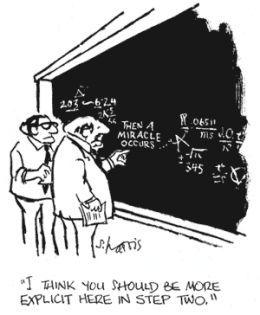
\includegraphics[width=\textwidth]{images/5ac7f04fdd13a8f6d8bc5396e1cf5812--math-jokes-math-humor.jpeg}
            {\scriptsize Prozess der Kalten Fusion}
            \end{center}
        \end{column}
    \end{columns}
    
    \vfill
    
    \begin{center}
    Vielen Dank für eure Aufmerksamkeit!
    \end{center}
    
    \vfill
\end{frame}

    \begin{frame}[allowframebreaks]{Literatur}
        \bibliographystyle{babalpha}
        \bibliography{bib.bib}
    \end{frame}
\end{document}
